\documentclass{beamer}

\usepackage[utf8]{inputenc}
\usepackage[brazil]{babel}
\usepackage{braket}

\title{Practical Byzantine Fault Tolerance}
\subtitle{Apresentação para a disciplina MATA88}
\author{Gabriel Dahia, Pedro Vidal}
\date{21 de Fevereiro de 2018}
\institute{Universidade Federal da Bahia}

\begin{document}

\frame{\maketitle}

\begin{frame}
  \frametitle{Introdução}
  \framesubtitle{Problema}

  \begin{itemize}
    \item
      Aumento da dependência de serviços online;

    \item
      Erros em software decorrentes da complexidade do software;

    \item
      Ataques maliciosos e erros ocasionam falhas bizantinas.
  \end{itemize}
\end{frame}

\begin{frame}
  \frametitle{Introdução}
  \framesubtitle{Contribuição}

  Um algoritmo prático para replicação de máquina de estados que tolera falhas bizantinas:
  \begin{itemize}
    \item
      Garante \textit{liveness} e \textit{safety};

    \item
      Funciona em sistemas assíncronos*;

    \item
      Não depende de sincronia para \textit{safety};

    \item
      Descreve otimizações que permitem uso prático;
      
    \item
      Performance superior à métodos anteriores.
  \end{itemize}
\end{frame}

\begin{frame}
  \frametitle{Modelo do Sistema}
  \framesubtitle{Comunicação}

  \begin{itemize}
    \item
      Sistema distribuído assíncrono;
      
    \item
      Nós são conectados por rede que pode:
      \begin{itemize}
        \item
          falhar em entregar mensagens;

        \item
          atrasá-las;

        \item
          duplicá-las; ou

        \item
          entregá-las fora de ordem.
      \end{itemize}
  \end{itemize}

\end{frame}

\begin{frame}
  \frametitle{Modelo do Sistema}
  \framesubtitle{Falhas}

  \begin{itemize}
    \item
      Modelo de falhas bizantinas;
      
    \item
      Exceção - nós falham independentemente:
      \begin{itemize}
        \item
          implementações diferentes por dispositivo;

        \item
          sistemas operacionais diversos; e

        \item
          senhas e administradores distintos.
      \end{itemize}
  \end{itemize}
\end{frame}

\begin{frame}
  \frametitle{Modelo do Sistema}
  \framesubtitle{Segurança}

  \begin{itemize}
    \item
      Criptografia para prevenir \textit{spoofing}, \textit{replays} e detecção de mensagens corrompidas;

    \item
      Técnicas que com alta probabilidade não podem ser subvertidas:
      \begin{itemize}
        \item
          Assinaturas de chave-pública;
          
        \item
          Códigos de autenticação; e
          
        \item
          Sumário de mensagens.
      \end{itemize}
  \end{itemize}
\end{frame}

\begin{frame}
  \frametitle{Modelo do Sistema}
  \framesubtitle{Adversário}

  \begin{itemize}
      \item
        Coordena nós comprometidos;

      \item
        Atrasa comunicação;

      \item
        Atrasa nós corretos não-indefinidamente.
  \end{itemize}
\end{frame}

\begin{frame}
  \frametitle{Propriedades do Serviço}

  \begin{itemize}
    \item
      Implementa qualquer serviço replicado com um \textbf{estado} e algumas \textbf{operações};

    \item
      Computações deterministícas arbitrárias;

    \item
      Clientes fazem requisições de invocação e bloqueiam esperando por uma resposta;

    \item
      Clientes e réplicas são corretos se seguem o algoritmo e suas assinaturas estão protegidas.
  \end{itemize}
\end{frame}

\begin{frame}
  \frametitle{Propriedades do Serviço}
  \framesubtitle{Resiliência ótima}

  \begin{figure}
    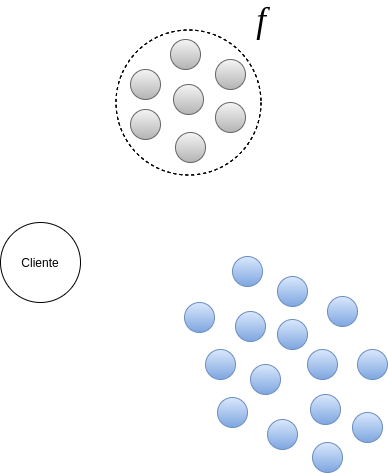
\includegraphics[width=0.5\textwidth]{images/resiliencia01}<1>
    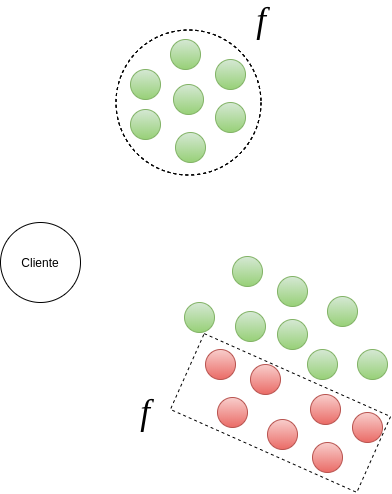
\includegraphics[width=0.51\textwidth]{images/resiliencia02}<2>
    \caption{Cliente faz requisição}
  \end{figure}

\end{frame}

\begin{frame}
  \frametitle{Propriedades do Serviço}
  \framesubtitle{\textit{Safety}}

  Funciona como se centralizado, executando operações atomicamente, uma por vez.
  \begin{itemize}
    \item
      Depende do número de réplicas que falham;

    \item
      Não depende de sincronia;

    \item
      Independe do número de clientes comprometidos;

    \item
      Não é protegido contra clientes maliciosos:
      \begin{itemize}
        \item
          Controle de acesso mitiga o problema.
      \end{itemize}
  \end{itemize}
\end{frame}

\begin{frame}
  \frametitle{Propriedades do Serviço}
  \framesubtitle{\textit{Liveness}}

  Cliente eventualmente recebe resposta.
  \begin{itemize}
    \item
      Depende de sincronia e retransmissões;
      
    \item
      Sincronia fraca: atraso não cresce mais rápido do que linearmente.
  \end{itemize}
\end{frame}

\begin{frame}
  \frametitle{Algoritmo}
  \framesubtitle{Definições}

  \begin{itemize}
    \item
      Máquinas de estados replicadas pelos nós;

    \item
      Cada máquina mantém o estado e implementa operações;

    \item
      Conjunto de réplicas $\mathcal{R}$, numeradas $0, ..., |\mathcal{R}| - 1$;

    \item
      $|\mathcal{R}| = 3f + 1$.
  \end{itemize}
\end{frame}

\begin{frame}
  \frametitle{Algoritmo}
  \framesubtitle{Definições}

  \begin{itemize}
    \item
      Sistema tem \textbf{visões}, $v$, consecutivas;

    \item
      Réplicas são:
      \begin{itemize}
        \item
          \textbf{primária} - se $p = v \text{ mod } |\mathcal{R}|$; ou
          
        \item
          \textbf{backups}.
      \end{itemize}

    \item
      Visão muda quando primária for suspeita.
  \end{itemize}
\end{frame}

\begin{frame}
  \frametitle{Algoritmo}
  \framesubtitle{Funcionamento}

  \begin{figure}
    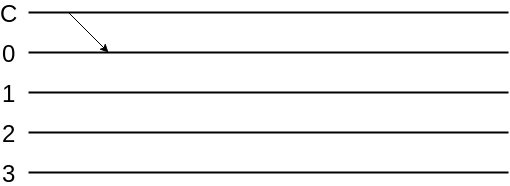
\includegraphics[width=0.75\textwidth]{images/algo01}<1>
    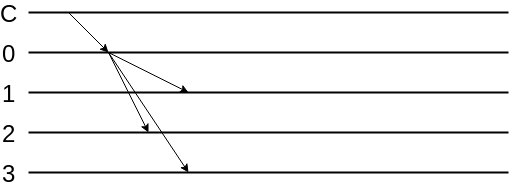
\includegraphics[width=0.75\textwidth]{images/algo02}<2>
    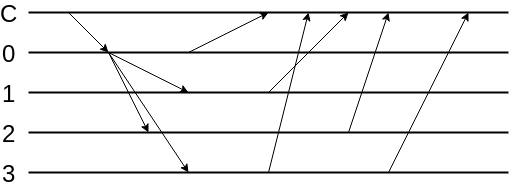
\includegraphics[width=0.75\textwidth]{images/algo03}<3>
    \caption{Esboço do funcionamento do algoritmo}
  \end{figure}
\end{frame}

\begin{frame}
  \frametitle{Algoritmo}
  \framesubtitle{Funcionamento}

  \begin{itemize}
    \item
      Réplicas precisam:
      \begin{itemize}
        \item
          ser determinísticas;

        \item
          começar no mesmo estado.
      \end{itemize}

    \item
      Todas as réplicas concordam em ordem total para execução, apesar de falhas.
  \end{itemize}
\end{frame}

\begin{frame}
  \frametitle{Algoritmo}
  \framesubtitle{Cliente}

  \begin{figure}
    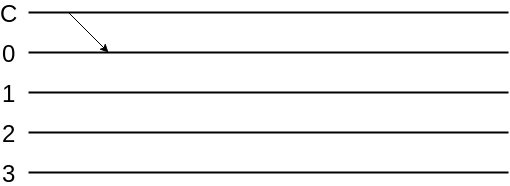
\includegraphics[width=0.75\textwidth]{images/algo01}
    \only<1>{\caption{Envia $\braket{\text{REQUEST}, o, t, c}{}_{\sigma_c}$}}
    \only<2>{\caption{Envia $\braket{\text{REQUEST}, \text{\alert{$o$}}, t, c}{}_{\sigma_c}$}}
    \only<3>{\caption{Envia $\braket{\text{REQUEST}, o, \text{\alert{$t$}}, c}{}_{\sigma_c}$}}
    \only<4>{\caption{Envia $\braket{\text{REQUEST}, o, t, \text{\alert{$c$}}}{}_{\text{\alert{$\sigma_c$}}}$}}
  \end{figure}
\end{frame}

\begin{frame}
  \frametitle{Algoritmo}
  \framesubtitle{Cliente}

  \begin{figure}
    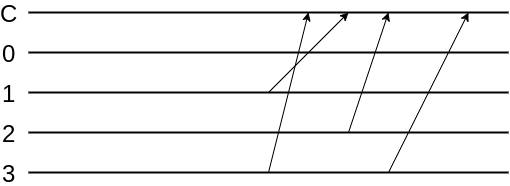
\includegraphics[width=0.75\textwidth]{images/client02}
    \only<1>{\caption{Réplicas respondem $\braket{\text{REPLY}, v, t, c, i, r}{}_{\sigma_i}$}}
    \only<2>{\caption{Réplicas respondem $\braket{\text{REPLY}, \text{\alert{$v$}}, t, c, i, r}{}_{\sigma_i}$}}
    \only<3>{\caption{Réplicas respondem $\braket{\text{REPLY}, v, \text{\alert{$t$}}, c, i, r}{}_{\sigma_i}$}}
    \only<4>{\caption{Réplicas respondem $\braket{\text{REPLY}, v, t, \text{\alert{$c$}}, i, r}{}_{\sigma_i}$}}
    \only<5>{\caption{Réplicas respondem $\braket{\text{REPLY}, v, t, c, \text{\alert{$i$}}, r}{}_{\text{\alert{$\sigma_i$}}}$}}
    \only<6>{\caption{Réplicas respondem $\braket{\text{REPLY}, v, t, c, i, \text{\alert{$r$}}}{}_{\sigma_i}$}}
  \end{figure}
\end{frame}

\begin{frame}
  \frametitle{Algoritmo}
  \framesubtitle{Cliente}

  \begin{figure}
    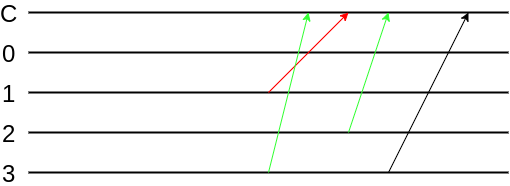
\includegraphics[width=0.75\textwidth]{images/client03}
    \caption{Cliente espera por $f+1$ respostas $\braket{\text{REPLY}, v, \text{\color{green} $t$}, c, i, \text{\color{green} $r$}}{}_{\sigma_i}$}
  \end{figure}
\end{frame}

\begin{frame}
  \frametitle{Algoritmo}
  \framesubtitle{Cliente}

  \begin{figure}
    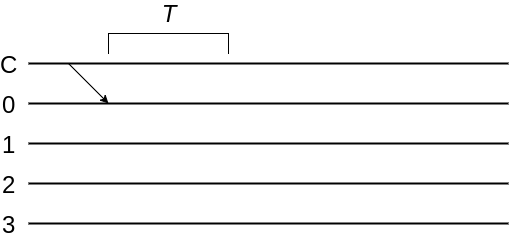
\includegraphics[width=0.75\textwidth]{images/client04}<1>
    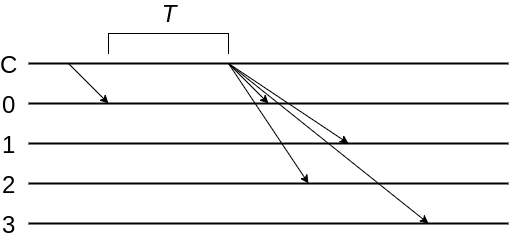
\includegraphics[width=0.75\textwidth]{images/client05}<2>
    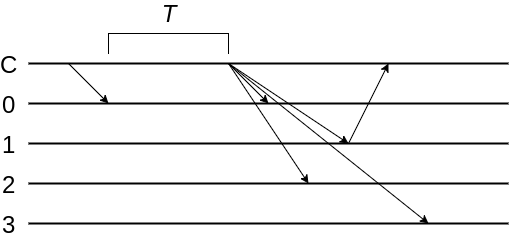
\includegraphics[width=0.75\textwidth]{images/client06}<3>
    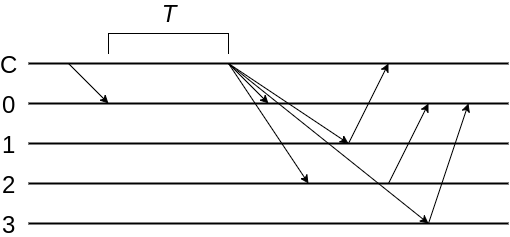
\includegraphics[width=0.75\textwidth]{images/client07}<4->
    \only<1>{\caption{Cliente dá \textit{timeout} esperando $f+1$ respostas}}
    \only<2>{\caption{Cliente faz \textit{broadcast} da requisição a todas as réplicas}}
    \only<3>{\caption{Réplicas que já tem $r$ reenviam ao cliente}}
    \only<4>{\caption{\textit{Backups} que ainda não tem, enviam requisição à primária}}
    \only<5>{\caption{Se primária não repassar ao grupo, será suspeita e visão mudará}}
  \end{figure}
\end{frame}

\end{document}
